\documentclass[12pt, A4]{article}
\usepackage{amsmath}
\usepackage[shortlabels]{enumitem}
\usepackage[margin = 0.75 in]{geometry}
\usepackage{tikz}
% Configuration
\title{Assignment 4}
\author{Arnav Patri}
% Notation
\newcommand{\pder}[2]{\frac{\partial #1}{\partial #2}}
\newcommand{\vi}{\text{\^\i}}
\newcommand{\vj}{\text{\^\j}}
\newcommand{\vk}{\text{\^k}}
\newcommand{\vps}{\hspace{0.5mm}}

\begin{document}
	\maketitle
		\begin{enumerate}[1)]
			\item
				Find and sketch the domain of the function $f(x, y) = \sqrt{x} + \sqrt{1 - x^2 - y^2}$.
				\begin{itemize}
					\item[] \textbf{Solution}
						\begin{align*}
							\sqrt{x} &\implies x \ge 0 \\
							\sqrt{1 - x^2 - y^2} &\implies x^2 + y^2 \le 1
						\end{align*}
						The latter equation is that of a circle, so the domain is simply the region bounded by the positive half of the circle $x^2 + y^2 = 1$.
						\[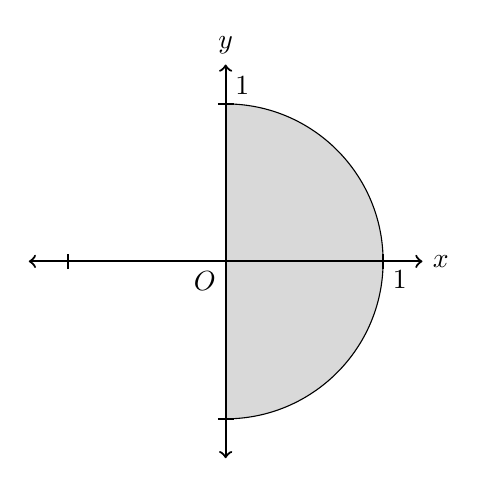
\begin{tikzpicture}[scale =2]
							\draw[fill = gray!30] (0, -1) arc[start angle = -90, end angle = 90, radius = 1cm];
							\draw[thick, <->] (-1.25, 0) -- (1.25, 0) node[anchor = west]{$x$};
							\draw[thick, <->] (0, -1.25) -- (0, 1.25) node[anchor = south]{$y$};
							\node at (0, 0) [anchor = north east] {$O$};
							\foreach \x in {-1, 1}
								\draw[thick] (\x, -0.05) -- (\x, 0.05);
							\foreach \y in {-1, 1}
								\draw[thick] (-0.05, \y) -- (0.05, \y);
							\node at (1, 0) [anchor = north west]{1};
							\node at (0, 1) [anchor = south west]{1};
						\end{tikzpicture}\]
				\end{itemize}
			\item
				Let $f(x, y) = 4 - x^2 - 5y^2$. Find $f_x(1, 1)$ and $f_y(1, 1)$ and interpret these numbers as slopes.
				\begin{itemize}
					\item[] \textbf{Solution}
						\begin{align*}
							f_x(x, y) &= -2x &
									f_y(x, y) &= -10y \\
							f_x(1, 1) &= -2(1) = -2 &
									f_y(1, 1) &= -10(1) = -10
						\end{align*}
						At the point where $x = 1$ and $y = 1$, the slopes of the lines tangent to $f(x, y) = 4 - x^2 - 5y^2$ parallel to the $x$- and $y$-axes respectively are $-2$ and $-10$.
				\end{itemize}

			\item
				Let $f(x, y) = x^3 + xy^2 - 3y^2$. Find $f_x$, $f_y$, $f_{xx}$, $f_{yy}$, and $f_{xy}$.
				\begin{itemize}
					\item[] \textbf{Solution}
						\begin{align*}
							f_x(x, y) &= 3x ^2 + y^2 &
									f_y(x, y) &= 2xy - 6y \\
							f_{xx}(x, y) &= 6x &
									f_{yy}(x, y) &= 2x - 6 \\
							f_{xy}(x, y) &= 2y
						\end{align*}
				\end{itemize}
			\item
				Find the equation of the tangent plane for $z = 3x^2 + y^2$ at $P(1, 1, z_0)$.
				\begin{itemize}[ ]
					\item \textbf{Solution}
						\begin{align*}
							z_0 &= 3(1)^2 + (1)^2
									= 4 \\
							\left.\pder{z}{x}\right|_{(x, y) = (1, 1)} &= 6x|_{(x, y) = (1, 1)} 
									= 6(1) 
									= 6 \\
							\left.\pder{z}{y}\right|_{(x, y) = (1, 1)} &= 2y|_{(x, y) = (1, 1)}
									= 2(1)
									= 2 \\
							z &= 6(x - 1) + 2(y - 1) + 4 \\
								&= 6x - 6 + 2y - 2 + 4 \\
								&= 6x + 2y - 4
						\end{align*}
				\end{itemize}
		\end{enumerate}
\end{document}
